\chapter{Transakční analýza}

Transakční analýza oproti ostatním psychologickým pohledům na
člověka se dívá na osobnost člověka z pohledu komunikace, 
z pohledu interpersonálních vztahů mezi jedinci. 
Tyto vztahy jsou opakující se, víceméně trvalé, přímé a 
nezprostředkované mezi dvěma lidmi či malou skupinou lidí a 
současně jsou provázeny emocionálním prožitkem ať už pozitivním či negativním \cite{interpersonalni_vztahy_slovnik}. Základním kamenem transakční analýzy je transakce, což je jednotka komunikace, která se skládá z podnětu a reakce \cite{transakcni_analyza_cata}. Transakce nemusí být verbální, může se jednat i o neverbální komunikaci.

Na počátku teorie transakční analýzy stojí tři základní potřeby:

    \begin{itemize}
        \item hlad po podnětech
        \item hlad po struktuře/organizaci času
        \item hlad po pozici
    \end{itemize}
    
{\it Hlad po podnětech} vede k vyhledávání různých vztahů a sociálních kontaktů. 
Naopak neuspokojení této potřeby může vést k rozvoji duševních poruch až k degenerativním změnám nervových buněk \cite{jak_si_lide_hraji}. 
Uspokojení tohoto hladu vede k interakcím tzv. {\it transakcím}.\\

{\it Hlad po struktuře/organizaci času} způsobuje, že lze veškeré lidské chování a prožívání rozčlenit do sedmi skupin dle struktury času a prostoru při tomto chování. 
Skupiny se liší mírou osobní pohody a společenské prospěšnosti. 
Člověk musí svým interakcím dát nějaký strukturovaný prostor, ve kterém se transakce budou odehrávat. 
Nemá-li čas strukturu, tak se člověk nudí. 
Má-li čas strukturu chaotickou, dostavují se úzkosti a neklid a také negativní transakce.\\

Typy transakcí dle struktury času: \textbf{zůstávání stranou, rituály, tlachání, hry (psychohry), práce, zábava, intimita}. V tomto pořadí jsou seřazeny od nejméně prospěšných po ty nejvíce pohodové \cite{translacni_analyza_prirucka}.\\

\subsubsection*{Zůstávání stranou}
Takový člověk se vyhýbá jakýmkoliv transakcím. Může tak působit povýšeně, ale ve skutečnosti jde o nešťastného člověka, který nedovede najít cestu k druhým.

\subsubsection*{Rituály}
Rituály jsou formalizované zavedené transakce. 
Pravděpodobně lidem šetří energii, současně umožňují se neotevírat se světu, mohou skrývat neupřímnost. 
Jde o formu obrany před intimními transakcemi, které ale působí, že máme o druhé zájem. 
Může se jednat o formu pozdravu nebo o chování při nějaké situaci.

\subsubsection*{Tlachání}
Je sled transakcí, které jsou více spontánní než rituály, ale také zabraňují jedincům ve vzniku intimních transakcí. Forma tlachání se velmi liší v závislosti na pohlaví a věku, ale také na vzdělání. Tyto interakce nemají za cíl vyřešit nějaký problém, ale jen nechat čas volně plynout. Případně ukázat jak máme nad druhým navrh (v čem jsme dobří). 

\subsubsection*{Hry}
Často jsou také označovány jako psychohry, ve většině případů mají negativní, destruktivní charakter. Cílem je získat výhodu nad druhým člověkem. Současně, ale pro některé lidi může být ziskem i pocit zmaru či ponížení. Těmto transakcím se budu dále věnovat v samostatné kapitole.

\subsubsection*{Práce nebo činnost}
Tento typ transakcí bývá pružný, jedinci v něm často zakouší sounáležitost a pozitivní emoce. Cílem transakcí bývá konkrétní vyřešení problémů.

\subsubsection*{Zábava}
Tyto transakce člověku většinou přináší radost, úlevu a odpočinek.
Může se jednat o posezení s přáteli, ale také o práci na zahradě či malování, není nutné, aby u zábavných transakcí byli dva lidé.

\subsubsection*{Důvěrný stav neboli intimita}
Tyto typy transakcí jsou pro jedince nejvíce obohacující. 
Jde o interakce s důvěrnými jedinci, o sdílenou vzájemnost, opravdovost a bezprostřednost.\\

\subsection*{Struktura stavů osobnosti}

Základní součástí transakcí a jejich analýzy je dále určení stavu osobnosti během transakcí. 
Transakční analýza rozlišuje tři ego-stavy: {\it rodič, dospělý a dítě} \cite{transakcni_analyza_cata}.
Jednoduchými přímými vztahy rozumíme v transakční analýze vztahy dvou jednotlivců, kteří se vyskytují v jednom ego-stavu. Pro tyto transakce lze vytvořit názorné vztahové diagramy, jak ukazuje obrázek \ref{fig:diagram_vztahu}. Vodorovné směry spojnic v diagramech označují vztahy {\it symetrické}, ostatní spojnice označují vztahy {\it asymetrické} \cite{sex_v_lidskem_milovani}. 

    \begin{figure}[h]
        \centering
        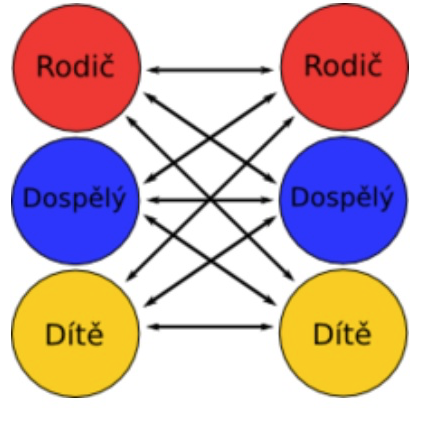
\includegraphics[width=0.7\textwidth]{pictures/diagram_vztahovy.png}
        \caption{Diagram vztahů, symetrické i asymetrické vztahy. \cite{everesta}}
        \label{fig:diagram_vztahu}
    \end{figure}{}

Jednoduchých přímých vztahů se účastní pouze jeden ego-stav. 
Jednoduché nepřímé vztahy jsou takové, kde se transakce účastní na každé straně jeden ego-stav, ale těsně před ním proběhl interní dialog s jiným ego-stavem. 
Těmto situacím se odborně říká {\it naprogramování}. 
Poslední skupinou jsou složené vztahy. Těchto transakcí se účastní více než dvě aktivní ego-stavy. 
Ve společenském měřítku se může jednat o intimní a dlouhodobé vztahy. 
Složené vztahy vedou častěji k nedorozumění, kříženým transakcím a hrám, 
současně ale mají vyšší šanci na přežití než vztahy jednoduché \cite{sex_v_lidskem_milovani}.\\

    \subsubsection*{Rodič}
    Jedná se o druh napodobování známé autority, nejčastěji rodiče, vychovatele, učitele. Rozlišujeme dva typu\cite{translacni_analyza_prirucka, socialni_psychologie_pro_pedagogy}:
        \begin{itemize}
            \item Kritický rodič - jedná s druhými tvrdě, u pedagogů převládá tendence žáky dirigovat, trestat, ovládat na úkor jejich samostatnosti. U druhých často provokuje vzdorné dítě.
            
            \item Pomáhající rodič - je laskavý, ochraňující, má tendenci ostatním vše všemožně usnadňovat. V druhých těší bezradné dítě.
        \end{itemize}{}
    
        
    \subsubsection*{Dítě}
    Jedná se o reprodukci svého vlastního dětského chování, schématickou reprodukci naučeného chování přibližně do pěti let věku. Hlavní vlastností dítěte je emotivnost. Rozlišujeme  čtyři typy \cite{translacni_analyza_prirucka, socialni_psychologie_pro_pedagogy}:
        \begin{itemize}
            \item Přirozené dítě - je zvídavé, dychtivé, bezprostřední a impulzivní, vyjadřuje věci bez zábran, má nízkou hranici brát věci vážně.
            
            \item Bezradné dítě - v tomto ego-stavu jsou všechny zážitky kritiky, trestů a zákazů. Toto dítě reaguje bezradně, hroutí se, zmatkuje, bojí se, pociťuje nejistotu a úzkost.
            
            \item Vzdorné dítě - má sklon vždy oponovat, je neschopné dojít ke konsenzu, přijmout názory druhých a dívat se na věci s nadhledem.
            
            \item Způsobné dítě - má sklon k vyhlížení autorit, jeho schématem je dosahování cíle vzorným chováním a poslušností. Způsobné dítě je ale méně tvořivé a bezprostřední.
        \end{itemize}{}
    
    
    \subsubsection*{Dospělý} 
    Tento ego-stav je zralou osobností, která se vymanila z reproduktivních tendencí. Pomocí dospělého jedinec poznává svět, klade otázky, řeší problémy, analyzuje, myslí, zvažuje alternativy, vytváří hypotézy, dokáže nezaujatě posuzovat komunikační partnery i sebe sama ve vzájemných vztazích. Dospělý je věcný, realistický, schopný růstu a zdokonalení \cite{translacni_analyza_prirucka, socialni_psychologie_pro_pedagogy}\\

\newpage

{\it Hlad po pozici} doprovází hlad po struktuře. 
Společnost očekává, že se budeme chovat v souladu s určitou pozicí, zajetým chováním. 
Pozice je způsob prožívání a chování vázané na dané podmínky. 
Tento hlad vysvětluje, proč je těžké pro jedince vykročit ze zajetých kolejí, protože i když sám chce projít velkou změnou, jeho okolím může tato změna být odmítána. 
To vysvětluje, proč jedinci často setrvávají i v jinak nevýhodných  a nepohodlných sociálních pozicích \cite{everesta}. 
Transakční analýza rozeznává čtyři pozice, které rozpracoval Thomas Anthony Harris ve svojí knize "Jsem OK, jste OK".
    
    \begin{itemize}
        \item Já jsem OK - Ty jsi OK
        \item Já nejsem OK - Ty jsi OK
        \item Já jsem OK - Ty nejsi OK
        \item Já nejsem OK - Ty nejsi OK
    \end{itemize}{}

Tyto základní životní pozice ovlivňují prožívání, myšlení a chování jednotlivce. Předpokládá se, že tyto stavy, které odrážejí celkový pocit vlastní hodnoty a hodnoty ostatních lidí jsou utvářeny v raném dětství na základě dětské zkušenosti \cite{transakcni_analyza_cata}. Transakční analýza uznává, že člověk se může na základě podmínek, ve kterých se pohybuje nacházet v různých životních pozicích \cite{translacni_analyza_prirucka}.




